%                                                                 aa.dem
% AA vers. 8.2, LaTeX class for Astronomy & Astrophysics
% demonstration file
%                                                       (c) EDP Sciences
%-----------------------------------------------------------------------
%
%\documentclass[referee]{aa} % for a referee version
%\documentclass[onecolumn]{aa} % for a paper on 1 column
%\documentclass[longauth]{aa} % for the long lists of affiliations
%\documentclass[rnote]{aa} % for the research notes
%\documentclass[letter]{aa} % for the letters
%\documentclass[bibyear]{aa} % if the references are not structured
% according to the author-year natbib style

%
\documentclass{aa}

%
\usepackage{graphicx}
%%%%%%%%%%%%%%%%%%%%%%%%%%%%%%%%%%%%%%%%
\usepackage{txfonts}
%%%%%%%%%%%%%%%%%%%%%%%%%%%%%%%%%%%%%%%%
\usepackage{hyperref}
\hypersetup{pdfborder=0 0 0, colorlinks=true, linkcolor=black, urlcolor=blue,
citecolor=black}
% To add links in your PDF file, use the package "hyperref"
% with options according to your LaTeX or PDFLaTeX drivers.
%
\renewcommand{\thefootnote}{\fnsymbol{footnote}}
\newcommand{\Sun}[0]{\ensuremath{_{\odot}}}
\newcommand{\mytilde}{\raise.17ex\hbox{$\scriptstyle\mathtt{\sim}$}}
\begin{document}


   \title{Simulating Stellar Evolution with AMUSE}

   \subtitle{Computational Astrophysics (CA) assignment two}

   \author{T. Halbesma (1603221)
          \inst{1}
          \and
          S. Sultan (1617451)\inst{2}
          }

   \institute{Anton Pannekoek Instituut (API), University of Amsterdam,
              Science Park 904, 1098 XH Amsterdam
              \email{timo.halbesma@student.uva.nl}
         \and
             Informatics Institute, Section Computational Science, University of Amsterdam,
             Science Park 904, 1098 XH Amsterdam
             \email{shabaz.sultan@student.uva.nl}
             }

   %\date{Received September 15, 1996; accepted March 16, 1997}

% \abstract{}{}{}{}{}
% 5 {} token are mandatory

  \abstract
  % context heading (optional)
  % {} leave it empty if necessary
   {}
  % aims heading (mandatory)
   {}
  % methods heading (mandatory)
   {}
  % results heading (mandatory)
   {}
  % conclusions heading (optional), leave it empty if necessary
   {}

   \keywords{Stellar Evolution --
                AMUSE --
                MESA -- EVTwin
               }

   \maketitle
%
%________________________________________________________________

\section{Introduction}
Once upon a time there was a star. The star was living quietly and peacefully whilst maturing. The evolution of this star has had and will have a profound effect on the life on Earth as this star is our Sun. The inhabitants of planet Earth were quite eager to known how the star were to evolve and how much more trouble- and worry free days our civilization would have left on our beloved habitat, our paradise Earth. A major reason to study stellar evolution is self preservation. Over the previous century much progress in this field has been made in understanding the equations governing the stellar structure and evolution. Additionally, over the last decade the computational power has increased drastically allowing for detailed calculations of, for instance, the Solar structure and (future) evolution using the previously acquired theoretical knowledge. With the current computing power at hand, one no longer has to assume stars to be static. For instance, we are now able to numerically calculate gravitational systems over the nuclear timescales of stars, also accounting for the stellar evolution that is expected to happen in astrophysical systems on this timescale.

In this report, the authors have used the Astrophysical Multipurpose Software Environment, in short AMUSE \citep{2009NewA...14..369P, 2013CoPhC.183..456P, 2013A&A...557A..84P}. As part of AMUSE several community codes are readily available by just changing a single code line. This allows for swift comparison between stellar evolution codes. Moreover, AMUSE combines gravitational dynamics code, stellar evolution methods and hydrodynamical algorithms. One of the great strengths of AMUSE is this combination enabling to set up a bridge between gravitational dynamics and stellar evolution routines. At first, in Sec.~\ref{sec:algorithms} we compare four stellar evolution algorithms. Next, in Sec.~\ref{sec:isochrones}, we obtain theoretical Hertzsprung–Russell diagrams for a given cluster age, so-called isochrones. We fit the isochrones to observed color-magnitude diagrams of clusters Hyades and Pleiades. We continue by examining the mass loss rate due to stellar evolution in Sec.~\ref{sec:massloss}. Finally, we set up the bridge between the stellar evolution and gravitational dynamics code to simulate clusters more realistically in Sec.~\ref{sec:SE_GD}, albeit with the significant simplifications casu quo assumptions discussed in Sec.~\ref{sec:discussion}. Finally, we present the conclusions in Sec.~\ref{sec:conclusions}

\section{Code Comparison}\label{sec:algorithms}
On the one hand we use two Henyey-type codes: \textbf{MESA} \citep{2011ApJS..192....3P, 2013ApJS..208....4P} and \textbf{EVTwin} \citep{1971MNRAS.151..351E, 1972MNRAS.156..361E, 1973MNRAS.163..279E, 1973A&A....23..325E, 1994MNRAS.270..121H, 1995MNRAS.274..964P, 2001ASPC..229..157E, 2001ApJ...552..664N, 2002ApJ...575..461E, 2007A&A...464L..57S, 2004MNRAS.348..201E, 2008A&A...488.1007G}. On the other hand, we use two parameterized codes:  \textbf{SSE} \citep{2000MNRAS.315..543H} and \textbf{SeBa} \citep{1996A&A...309..179P, 2012A&A...546A..70T}. For a detailed explanation of the Henyey-type code we refer the reader to \cite{1959ApJ...129..628H}. As for parameterized code, we cite \cite{AMUSEdocumentation}: ``stars are parameterized by mass, radius, luminosity, core mass, etc. as functions of time and initial mass''. The star is evolved from zero-age main sequence onwards to obtain the model parameters. The algorithms are analytic fit-based which makes SSE and SEBA rapid. Table~\ref{tab:algorithms} shows a comparison of general properties for the different algorithms.

In our analysis, we will evolve a star of solar mass and solar metallicity up to the current age of the Sun of 4.57 $\pm$ 0.11 Gyr \citep{2002A&A...390.1115B}. By default, the stellar evolution codes in AMUSE assume that the solar metallicity $z = 0.02$.
In addition, we will run a simulation of a star with 10 M\Sun up to 30 Myr because we expect heavier stars to evolve more rapidly. Specifically, the expected main sequence (hydrogen burning) lifetime $\tau_H$ as a function of mass is given by \citep[][p. 347]{2012sse..book.....K}. Normalised to the Solar lifetime of 10 Gyr \citep{1993ApJ...418..457S} yields
\begin{eqnarray}
     \tau_H(M) = 10^{10} \cdot \left(\frac{M}{M\Sun}\right)^{-2.5},
\end{eqnarray} where $M$ is the mass of the star. For a 10 solar mass star we expect the star to stay on the main sequence when it is evolved until 30 Myr.

Table~\ref{tab:parameterspace} shows the input parameters and the results for the for different algorithms. Three interesting observations are made. Firstly, $L$, $M$ and $R$ are of order unity in solar units, as expected for solar evolution up to the current age of the Sun, save for the final stellar radius calculated using the EVTwin algorithm. This is attributed to a potentially failed build of the EVTwin algorithm which causes suspision in using the EVTwin algorithm. Secondly, the Henyey model calculation times are significantly larger than the parameterized algorithms. In this case, the Henyey runtime is an order of magnitude larger than the parameterized runtime. Lastly, SSE and SeBa yield the same results. This is not surprisingly as the algorithms are not expected to differ for one star because SeBa is a more eleborate algorithm consisting of both SSE and binary evolution code.

\begin{table*}
    \caption{General properties of the Stellar Evolution codes \citep{AMUSEdocumentation}}
    \label{tab:algorithms}
    \centering
    \begin{tabular}{l l l l l l l l }
        \hline\hline
        Algorithm & Type & Binary/Single & Metallicity $z$ & Mass $m$ (M\Sun) \\
        \hline
        MESA & Henyey & Both & All, even 0 & 0.1 - 100 \\
        EVTwin & Henyey & Single\footnotemark[1] & 0.02 only & ? \\
        SSE & Parameterized & Single & 0.0001 - 0.03 & 0.1 - 100 \\
        SeBa & Parameterized & Both & 0.0001 - 0.03 & 0.1 - 100 \\
        \hline
    \end{tabular}
\end{table*}
\addtocounter{footnote}{1}
\footnotetext[\value{footnote}]{Binaries are not yet available in AMUSE EVTwin Interface.}

\setlength\tabcolsep{2pt}
\begin{table}
    \caption[]{Parameters and results of simulations. Here, $z$ is the metallicity, $t_{\rm end}$ the end time of the simulation, $L$ the luminosity, $M$ the mass, $R$ the radius and Runtime is the wall-clock runtime of the algorithm.}
    \label{tab:parameterspace}
    \begin{tabular}{lcccccc}
        \hline
        \noalign{\smallskip}
        Algorithm & $z$ & $t_{\rm end} (Myr)$ & $L$ (L\Sun) & $M$ (M\Sun) & $R$ (R\Sun) & Runtime (s) \\
        \hline
        \noalign{\smallskip}
        MESA & 0.02 & 4600 & 1.034 & 1 & 1.016 & 9.54 \\
        EVTwin  & 0.02 & 4600 & 1.027 & 1 & 0.1834 & 9.58 \\
        SeBa & 0.02 & 4600 & 0.9585 & 1 & 0.9856 & 0.554 \\
        SSE & 0.02 & 4600 & 0.9585 & 1 & 0.9856 & 0.166 \\
        MESA & 0.02 & 30 &  &  &  &  \\
        EVTwin & 0.02 & 30 &  &  &  &  \\
        SeBa & 0.02 & 30 &  &  &  &  \\
        SSE & 0.02 & 30 &  &  &  &  \\
        \hline
        \noalign{\smallskip}
        \noalign{\smallskip}
    \end{tabular}
\end{table}

\section{Cluster age}\label{sec:isochrones}
The method used to calculate the age of the Hyades and Pleiades clusters is described in this section. Firstly, a set of $N$ stars following an initial mass function (IMF) is generated, where $N$ is the number of stars that we set equal to the amount of data points in the dataset. The Hyades dataset consists of 1339 measured stars and Hyades has 887 data entries. Here we adopt the empirically derived Salpeter IMF \citep{1955ApJ...121..161S} given by
\begin{eqnarray}
    \zeta(m) \Delta m = \zeta_0 \left(\frac{m}{M\Sun}\right)^{\alpha} \left(\frac{\Delta m}{M\Sun}\right),
\end{eqnarray} where the exponent $\alpha = -2.35$. In AMUSE the SalpeterIMF implementation yields a mass within the range 0.1 - 125 M\Sun. The IMF shows clearly that higher mass stars are more rare, which we expect. Using this stellar population, generated at the same point in time, we start the stellar evolution using the SSE algorithm for a given metallicity. We adopt $z = 0.14$ \citep{1998A&A...331...81P} as Hyades metallicity, and for the Pleiades we assume $z = 0.02$ because we could not find a metallicity value in the literature.

    Next, we obtained observed color-magnitude diagrams of the Hyades and Pleiades cluster from the online version of the database for galactic open clusters, BDA \citep{1995ASSL..203..127M}, accessible at \citep{webda}. These photometric datasets contain observed apparent magnitudes in the V band and values of B-V. A measure of the `reddening' of 0.010 magnitude is provided by WEBDA for the Hyades, but no measure of the reddening is available for the Pleiades. This reddening might be a measure of the interstellar extinction but, since we were unsure and we only have a value for one cluster, we did not include this value in the analysis. 

    To allow for fitting of the numerically calculated HR diagrams, the color-magnitude measures have to be converted to luminosity and $T_{\rm eff}$. Alternatively, the numerical luminosity may be converted to apparent visual magnitude in the V-band and the effective temperature to a corresponding B-V value. We chose the former using equations~\eqref{eq:lum}~and~\eqref{eq:teff}. For the luminosity $L$ we find


\begin{eqnarray}
    \log \left(\frac{L_{\rm star}}{L\Sun}\right) = \frac{(M_{V,\rm star}-M_{V,\odot})}{-2.5} \left(\frac{d_{\rm star}}{d\Sun}\right)^2 \label{eq:lum},
\end{eqnarray}
where $M$ the observed apparent magnitude in the V-band and $d$ the distance. Here we adopt $M_{V, \odot} = -26.73$ \citep{1957ApJ...126..266S}. To obtain the temperature from B and V photometric filter measurements, we use the equation derived by \citet{2012EL.....9734008B}
\begin{eqnarray}
    T = 4600 \left(\frac{1}{0.92 (B-V) + 1.7} + \frac{1}{0.92(B-V) + 0.62} \right) \label{eq:teff}.
\end{eqnarray}

Fig.~\ref{fig:bestfit} shows the converted observations in red and the numerical values in green. In this particular plot we show the best fit. To determine which cluster lifetime fits best to the observations we first need to calculate to which simulated point of the HR diagram in the main sequence, giant branch or white dwarf the observed datapoint is the nearest. We do so using a nearest neighbour algorithm. Next, we calculate two $\chi^2$ values: one for the luminosity and one for the effective temperature. Since the order of magnitude of $\chi^2$ may differ for the luminosity and the effective temperature, we normalize these values such that they are comparable. We calculate $$\chi^2_{\rm normalized} = \sqrt{\frac{\sum_{i=0}^{\rm starcount} (T_i - T_{\rm average})^2}{i}}$$, where $T_i$ is the temperature of star, $T_{\rm average}$ is the temperature averaged over all times, and $i$ is the total number of stars in the dataset. This same formula is used for the luminosities.

Using the method described in the previous paragraph we have obtained Fig.~\ref{fig:chisq} showing the chi squared values for the cluster age in a range from 0 Myr to 1000 Myr. Note that initially our calculated $\chi^2$ is very low compared, then quickly rises, drops to a local minimum and then rises again. We contribute this behaviour to the fact from 0 to 200 Myr the heaviest stars are not yet evolved. This means that there are no stars in the giant branch and asymptotic giant branches. The luminosities are up to three decades higher for those stars causing the rise in $\chi^2$. Those stars either end as white dwarfs or go supernova, to create neutron stars or black holes. Once the white dwarfs start ascending to the lower left of the HR diagram, the main sequence begins to show show a turnoff towards the giant branches, and the giant branch just post Hertzspurung gap starts to be populated, $\chi^2$ decreases again. We expect the ZAMS turnoff point to be the most significant feature to determine the cluster age. To compare, Fig.~\ref{eq:ZAMS} clearly shows the ZAMS for a cluster of 0 Myr without a turnoff towards the giant branches. Moreover, the lower left corner contains no white dwarfs. Another interesting $\chi^2$ value is found at 810 Myr, where a single point breaks the trend. We discard this point for this reason and conclude that the age of the Hyades is 680 Myr. NB, this analysis has only been done once. To calculate a statistical average we would like to conduct the experiment multiple times using several Salpeter IMFs.

\begin{figure}
    \centering
    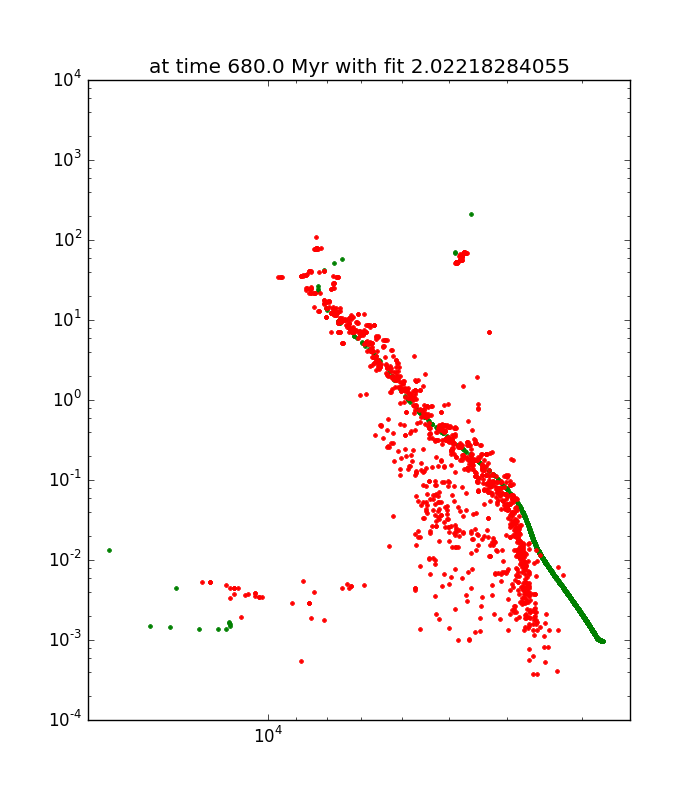
\includegraphics[width=\hsize]{img/test680.png}
    \caption{REPLACE}\label{fig:bestfit}
\end{figure}

\begin{figure}
    \centering
    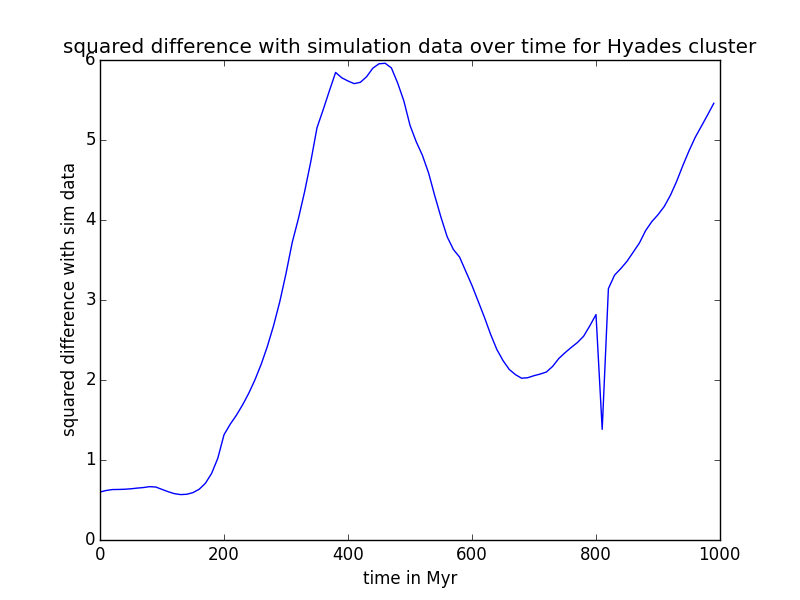
\includegraphics[width=\hsize]{img/fitness_over_time.png}
    \caption{REPLACE}\label{fig:chisq}
\end{figure}

\begin{figure}
    \centering
    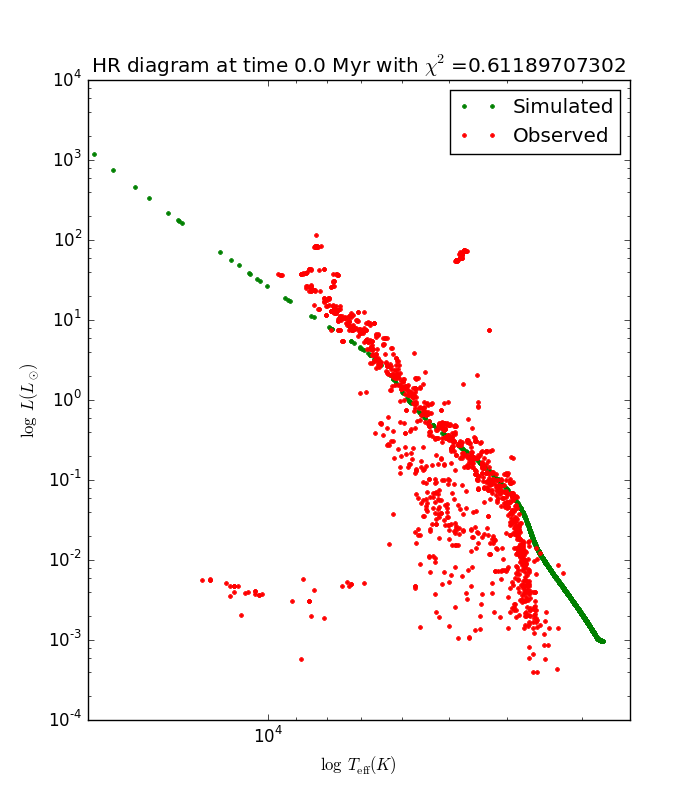
\includegraphics[width=\hsize]{img/test0.png}
    \caption{REPLACE}\label{fig:ZAMS}
\end{figure}


\section{Cluster mass-loss} \label{sec:massloss}
% \begin{figure}
%     \centering
%     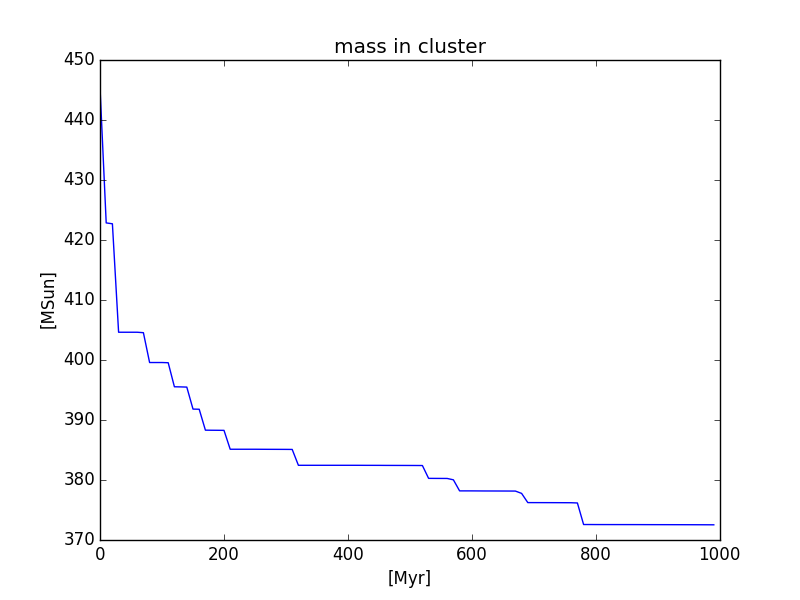
\includegraphics[width=\hsize]{img/mass_over_time.png}
%     \caption{REPLACE}\label{fig:mass_over_time
% \end{figure}
As stars age they loose mass. By simulating a group of stars with an appropriate distribution of different masses for the stars we can study how a cluster of stars changes in mass. The changing mass can have further repercussion for the gravitational interaction within a cluster (see section~\ref{sec:SE_GD}). 

We have initialized a set of stars with the Salpeter IMF. In figure~\ref{fig:massfraction} we can see that over a 1000 Myr simulation the cluster loses about 16\% of its mass. It should be noted that we are strictly talking about mass inside stars; clusters can have mass that is contained in things like dust and gas clouds. Specifically at 680 Myr (the age derived in section~\ref{sec:isochrones}) the fraction of mass retained in stars relative to the starting mass was 84\%. 

This simulation was done with parameters simulating the Hyades. The present day total mass of the Hyades cluster is about 400 M\Sun \citep{2009AIPC.1094..497B}. This would imply an initial cluster mass of $\frac{400 M\Sun}{0.84} \approx 476 M\Sun$ if we want to end up with a mass of 400 M\Sun at 680 Myr. 
\begin{figure}
    \centering
    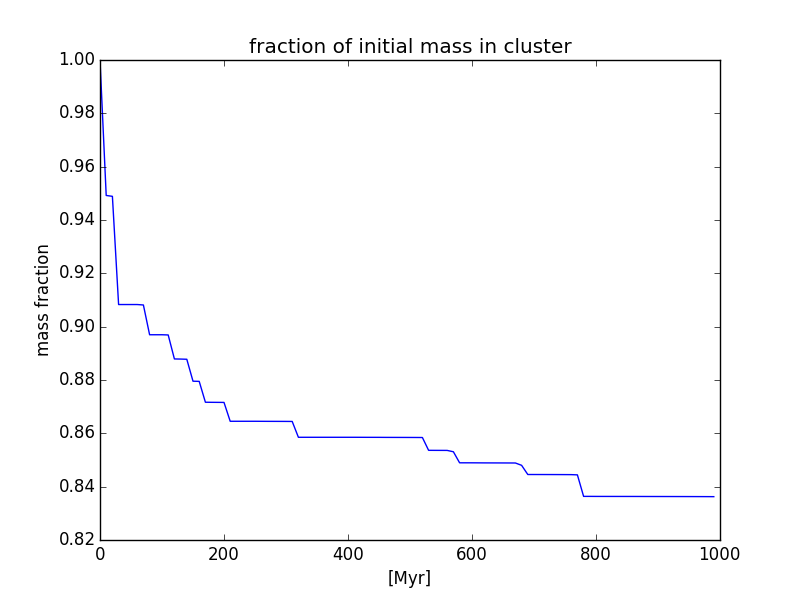
\includegraphics[width=\hsize]{img/massfraction_over_time.png}
    \caption{Fraction of initial mass present in stars of a cluster over time.}\label{fig:massfraction}
\end{figure}

\section{Stellar Evolution \& Gravitational Dynamics} \label{sec:SE_GD}
Clusters are groups of stars that to some extent are gravitationally bound to each other. Globular clusters can be quite tightly bound while open cluster can be bound somewhat more loosely. By simulating a cluster's gravitational interaction over time and finding how many stars remain bound we can study how strongly the stars are bound to the rest of the cluster and how this changes at different ages of the cluster. By using N-body codes the behavior of gravitationally bound and unbound stars can be studied computationally.

Just running an N-body code on a simulated cluster makes the implicit assumption that the stars are static objects in everything but position and velocity. In particular, it makes the assumption that the masses of the stars do not change. In reality stars change in mass as they progress through their life, which may have a significant impact on the way they gravitationally interact with the rest of a cluster.

We can integrate stellar evolution code with an N-body simulation to make our simulation more accurate. By simulating each star's evolution over time we can use this to determine the mass of each star over time. These masses can in turn be used as the input of an N-body code. By alternatingly simulating stellar evolution and gravitational interaction the N-body code will now use different masses for the same star over time.

We have run the simulation with the Barnes-Hut Tree N-Body simulation code for a total period of 1000 Myr. The stellar evolution code being used is SSE. The stellar evolution is run at 10 Myr increments. The N-Body code then takes the new masses and simulates the gravitational dynamics for 10 Myr as well, with a timestep of 0.1 Myr (i.e. it uses 100 timesteps to move the gravitational simulation forward by 10 Myr).

To find the stars that are considered gravitationally bound the HOP algorithm is used \citep{1998ApJ...498..137E}. Based on this algorithm the number of bound stars in the cluster can be seen in figure~\ref{fig:bound_stars}. The cluster only looses about 7 stars at the start of the simulation and stabilizes at 7-9 unbounded stars and over 1300 that remain bounded. 

Because the bound stars metric doesn't show a lot of change instead the clusters radius over time might be a more interesting metric. The most naive way to measure radius is to take the maximum distance a star has to the centre of the cluster. As can be seen in figure~\ref{fig:max_radius} this radius increases roughly linearly over time. Because it is determined by the outermost star, this would be consistent with a system where there is at least one star that is relatively unbound by the clusters gravity and is moving away from its centre at a roughly constant speed. 

More interesting is the virial radius. For our simulated cluster this was at 10 lightyears (about 3 parsecs), matching the core radius of the Hyades cluster \citep{2009AIPC.1094..497B}. As can be seen in figure~\ref{fig:virial_radius} it has a large jump at the star of the simulation and then a more slowly increasing trend.

Finally we can look at what phases of their lives the stars in the simulation are over time. We group the stars into three categories: main sequence stars, giant stars and remnant stars. In figure~\ref{fig:phases} it can be seen that the fast majority of the stars are on the main sequence and remain their during the simulation. When we only look at giant and remnant stars in figure~\ref{fig:phases_without_ms} we can see that while the number of remnant stars steadily increases, the number of giant stars at any single point in time remains relatively constant. This implies that the rate of stars entering their giant phase and burning out from the giant phase is roughly equal.
\begin{figure}
    \centering
    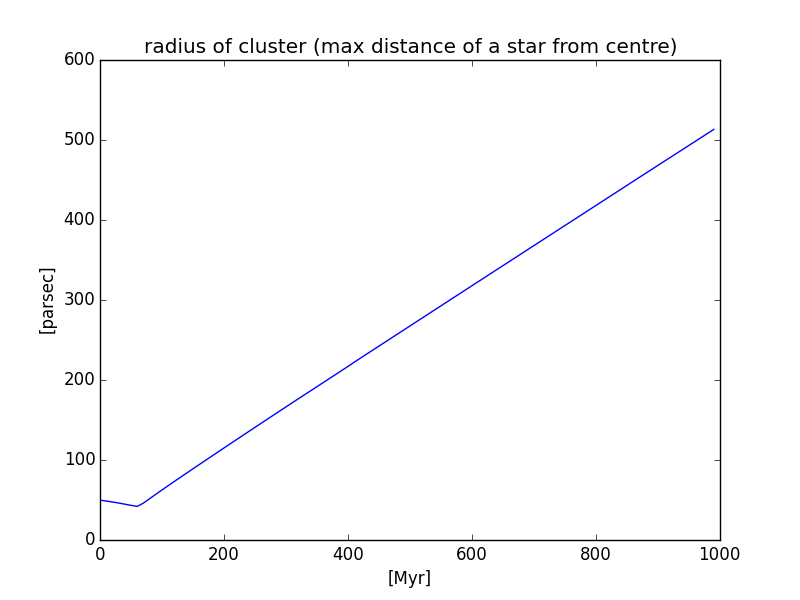
\includegraphics[width=\hsize]{img/cluster_max_radius.png}
    \caption{Radius of the cluster, determined by star furthest away from centre.}\label{fig:max_radius}
\end{figure}

\begin{figure}
    \centering
    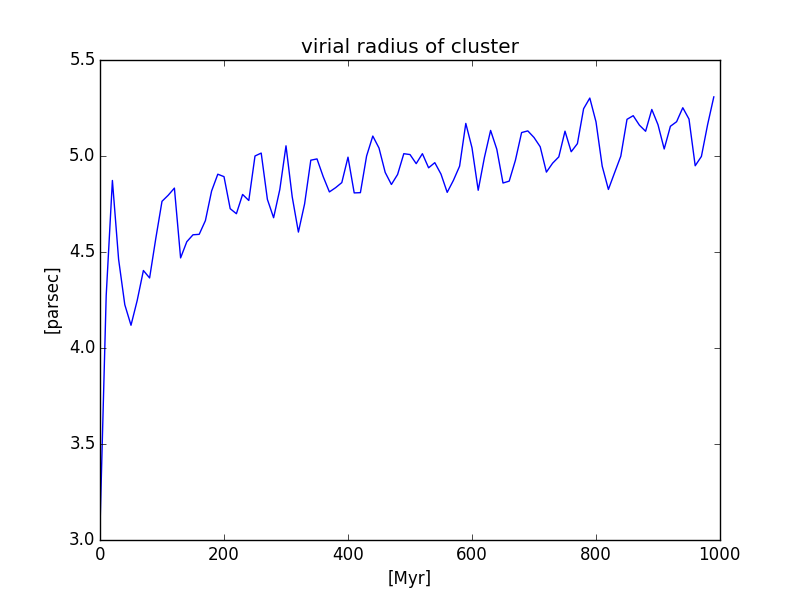
\includegraphics[width=\hsize]{img/cluster_virial_radius.png}
    \caption{Virial radius of cluster over time.}\label{fig:virial_radius}
\end{figure}

\begin{figure}
    \centering
    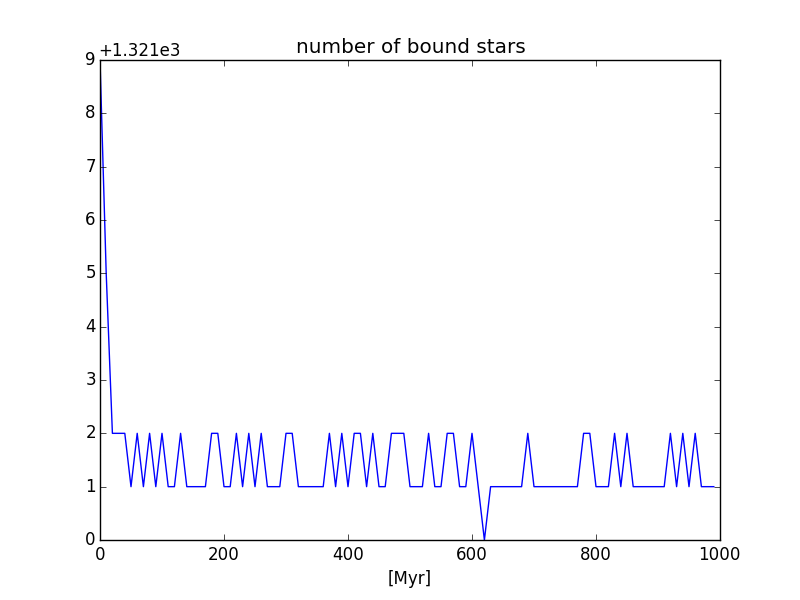
\includegraphics[width=\hsize]{img/bound_stars.png}
    \caption{Number of stars gravitationally bound by cluster.}\label{fig:bound_stars}
\end{figure}

\begin{figure}
    \centering
    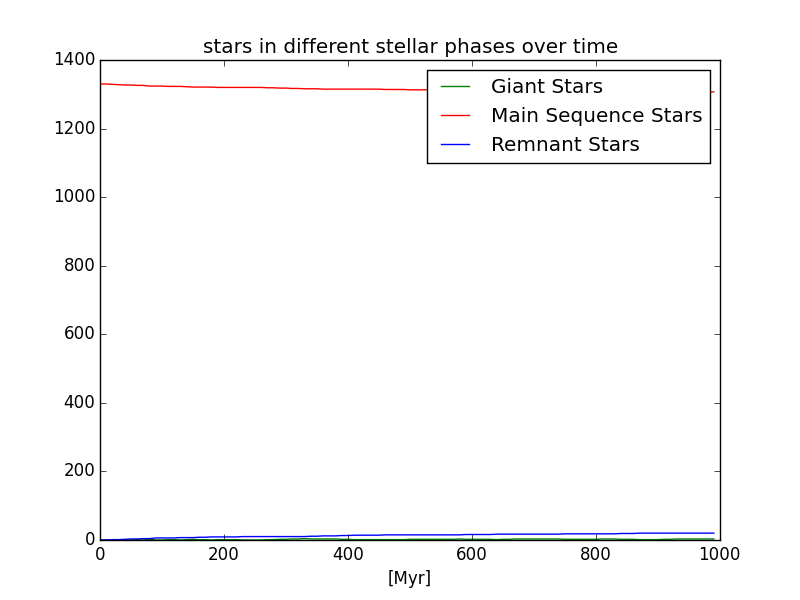
\includegraphics[width=\hsize]{img/stellar_phases_counts.png}
    \caption{Stars in three stellar evolution categories over time.}\label{fig:phases}
\end{figure}

\begin{figure}
    \centering
    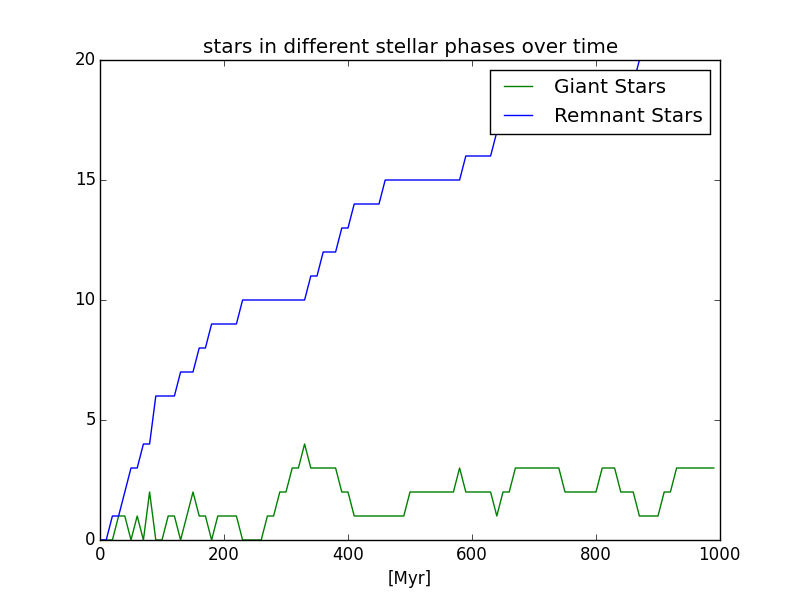
\includegraphics[width=\hsize]{img/stellar_phases_counts_without_main_sequence.png}
    \caption{Stars in two stellar evolution categories over time (excluding main sequence stars).}\label{fig:phases_without_ms}
\end{figure}

\section{Discussion}\label{sec:discussion}
We must assume that all stars in the cluster are formed at the same point in time in order to use this method. This assumption might not be true as observations show that star formation in clusters might be at different times, causing multiple populations in stellar clusters \citep{2009IAUS..258..233P}.

Binaries are not included in our analysis, although research has shown that almost one in three stars in the Milky Way is in a binary \citep{2006ApJ...640L..63L}. This is a significant fraction that should be included in the analysis.

We have assumed the stars to follow the Salpeter IMF. Other, more recent IMFs are available \citep[e.g.][]{1979ApJS...41..513M, 2001ASPC..228..187K, 2001MNRAS.322..231K} and may be taken into the analysis as a variable.
For instance, \citet{2001MNRAS.322..231K} is concerned that a universal initial mass function (IMF) is not intuitive yet evidence lacks to support of a variable IMF. Moreover, different slopes are introduced for stars below 0.08 M\Sun and between 0.08 M\Sun and 0.5 M\Sun. In our analysis, we have produced stars with masses below 0.5 M\Sun so this could influence the results. In fact, the mean mass of the Salpeter IMF is 0.35 M\Sun, which is in the 0.08 - 0.5 M\Sun mass range requiring an alternate power law index $\alpha$. This influence should be studied in depth but lacks in our analysis.

We would like to emphasize that the current value of the Solar metallicity is highly debated at present. AMUSE by defaults chooses $z = 0.02$ as Solar metallicity. This value lies within the range of possible Solar metallicities of $z= 0.0187$ to $z = 0.0239$ \citep{2007ApJ...670..872C}. Note, however, that three-dimensional hydrodynamical simulations of the Solar atmosphere yield a significantly lower solar metallicity of $z = 0.0122$ \citep{2006CoAst.147...76A}. At present, most stellar evolution models assume a one dimensional (spherically symmetric) geometry. This neglects three dimensional convective flows that might have a significant influence on the stellar structure. We did not perform a detailed analysis of different stellar metallicities and we merely state that the reader should be cautious regarding the Solar metallicity and note that we adopt $z = 0.02$ as the Solar metallicity because AMUSE defaults to said value. This discussion is highly relevant because, for example, metallicity has a profound influence on the stellar evolution \citep[e.g.][]{1960ApJ...131..598S}. Having said so, the metallicity for the Hyades has been obtained from the literature. We therefore state that for isochrone fitting of the Hyades the metallicity is not a point of discussion. Conversely, the metallicity of the Pleiades was not obtained from the literature, thus, is assumed to be Solar. This analysis might require redoing with a measured metallicity value.

We have noticed that the dataset has double entries. This occurs, for instance, when multiple publications governing the same star exist in the literature. Consequently, some stars have erroneously been given a higher weighing factor in the least squares determination.  We, however, neglect this because (e.g. in the Hyades dataset) we have found that most stars have double entries and stars with double entries span the entire spectrum. We therefore assume that this does not significantly influence the end-result. On the other hand, future analysis can be improved by averaging the data points and calculating the observational error to be used in the least squares averaging. This will result in improving the weight factor as observations contradicting each other will be given a lower weight factor whereas observations in agreement are given a higher weight factor due to the $chi^2$ calculations.

\section{Conclusions}\ref{sec:conclusions}

   \begin{enumerate}
      \item
      \item
   \end{enumerate}


\begin{acknowledgements}
The authors are grateful for the help of their supervisors Edwin van der Helm, MSc and Prof.dr. S.F. Portegies Zwart. \\

This research has made use of the WEBDA database, operated at the Department of Theoretical Physics and Astrophysics of the Masaryk University. \\

This research has made use of NASA's Astrophysics Data System.
\end{acknowledgements}


%-------------------------------------------------------------------

\bibliographystyle{aa}
%\setlength{\bibsep}{0pt} % Remove whitespace in bibliography.
\bibliography{CA_SE_TLRH_s1603221_SS_s1617451_report_aa}
\end{document}
